\setcounter{chapter}{0}
\chapter[Simulado 1]{Simulado}

\num{1} Os números distribuídos abaixo pertencem a dois conjuntos.

$A = \sqrt{2} \\ 
B = \frac{3}{5} \\ 
C = 0,454545\ldots{} \\
D = \sqrt{5}$

A distribuição dos conjuntos pode ser feita da seguinte maneira:

\begin{escolha}

  \item A e B pertencem aos Naturais, C e D pertencem aos Racionais.

  \item A e D pertencem aos Irracionais, B e C pertencem aos Racionais.
  
  \item A e C, pertencem aos Irracionais, B e D pertencem aos Racionais.
  
  \item A e D pertencem aos Racionais, B e C pertencem aos Irracionais.

\end{escolha}



\num{2} A distância média entre a Terra e o Sol é de aproximadamente 149,6
milhões de quilômetros. Essa distância é fundamental para a vida em
nosso planeta, pois determina a quantidade de energia solar que
recebemos. A Terra orbita ao redor do Sol em uma trajetória elíptica,
o que significa que a distância entre eles varia ao longo do ano. No
ponto mais próximo da Terra ao Sol, chamado de \textit{perigeu}, essa distância
pode ser de cerca de 147 milhões de quilômetros, enquanto no ponto
mais distante, chamado de \textit{apogeu}, pode chegar a cerca de 152 milhões
de quilômetros. Essas variações na distância não são significativas o
suficiente para afetar drasticamente a vida na Terra, mas podem ter
efeitos no clima e nas estações do ano.

A distância da Terra ao Sol no apogeu pode ser representada da seguinte maneira:

\begin{escolha}

  \item $1496 \cdot 10^{6}$ km 

  \item $14,96 \cdot 10^{6}$ km 

  \item $1,52 \cdot 10^{8}$ km 

  \item $152.000$ km

\end{escolha}

\num{3} Observando a malha:

\begin{figure}[htpb!]
\centering
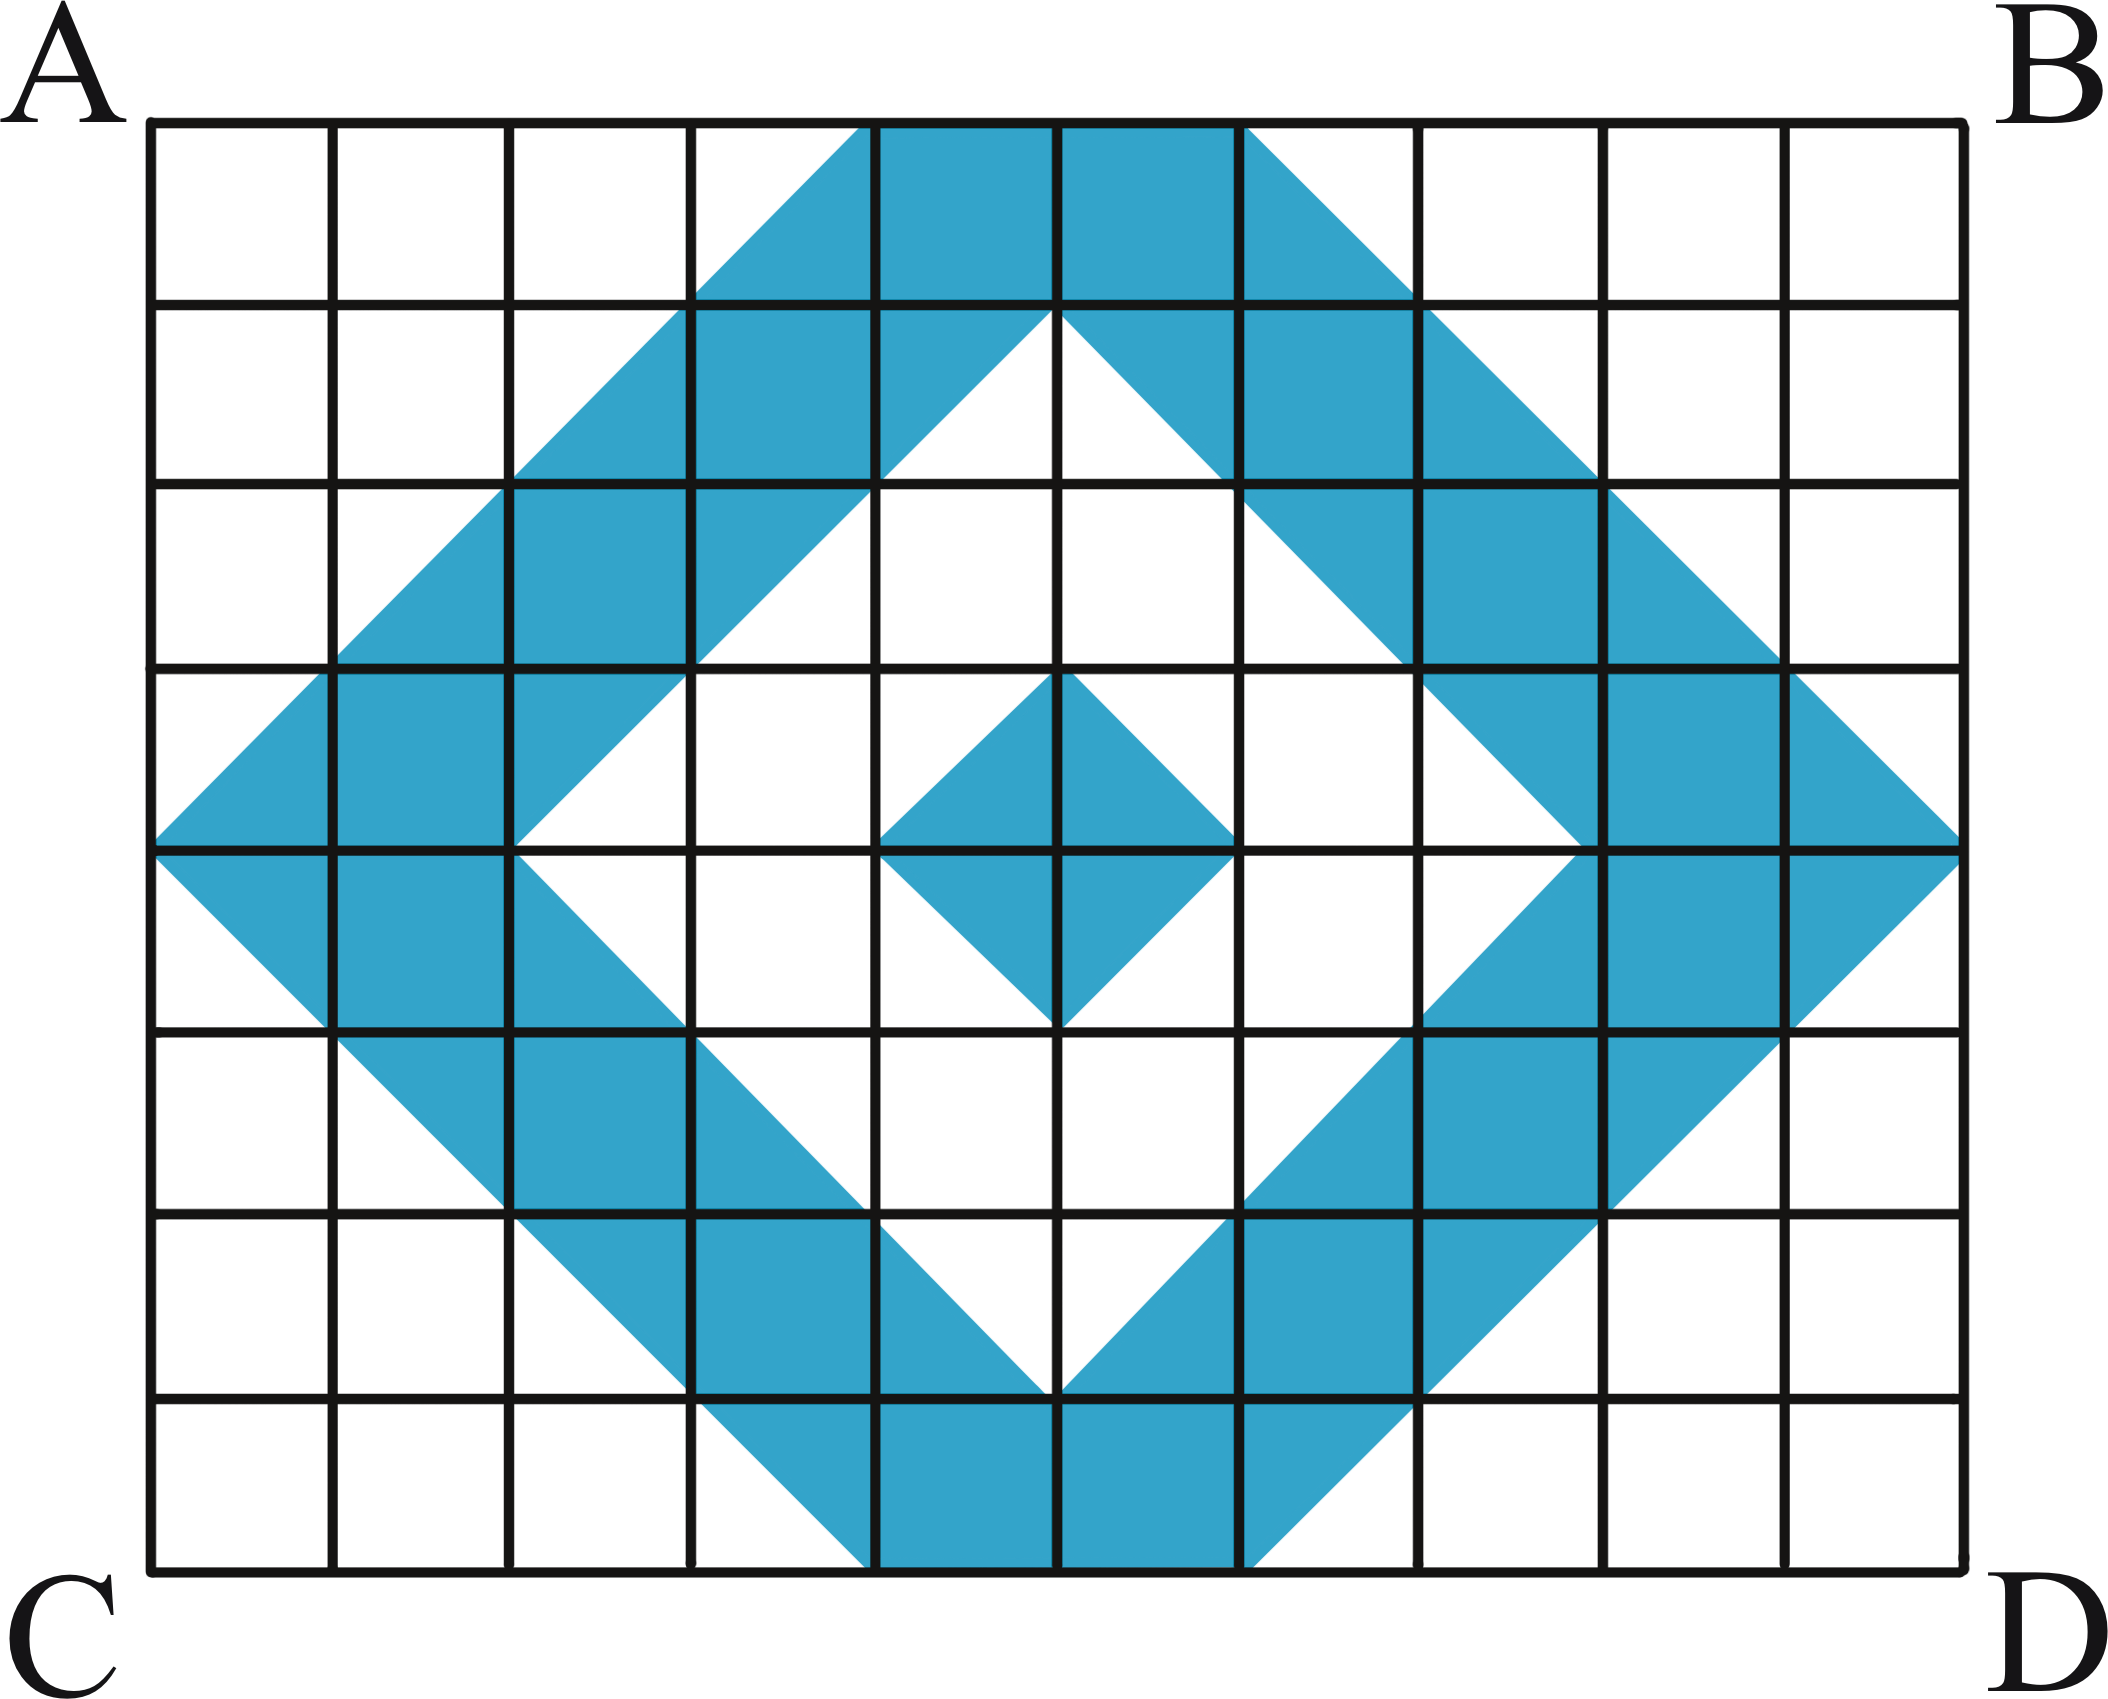
\includegraphics[width=.4\textwidth]{./ilustras-mat/Simulado_1-atividade_3.png}
\end{figure}

\pagebreak
Qual a fração da malha colorida em relação ao total?

\begin{escolha}

  \item $\frac{1}{5}$

  \item $\frac{2}{5}$

  \item $\frac{3}{5}$

  \item $\frac{4}{5}$

\end{escolha}

\num{4} Pedro tem uma dívida com o banco no valor de R\$ 6000,00. Neste mês
recebeu um bônus por desempenho e pagará 20\% desta dívida.

Qual valor ele pagará ao banco?

\begin{escolha}

  \item R\$ 120,00

  \item R\$ 1.000,00

  \item R\$ 1.200,00

  \item R\$ 2.400,00

\end{escolha}


\num{5} Aluísio olhou sua carteira e decidiu dar um terço do dinheiro 
que tinha para sua neta mais velha. Posteriormente ele deu mais 10 reais 
a ela e ficou com 20 reais na carteira.

Qual equação permite encontrar o valor que o avô Aluísio tinha na 
carteira?

\begin{escolha}

\item $\frac{x}{3} - 10 = 20$ 

\item $x - \frac{x}{3} - 10 = 20$ 

\item $x + 10 = \frac{x}{3} - 20$ 

\item $\frac{x}{3} - \frac{10}{3} = 20$ 

\end{escolha}

\num{6} Observe a imagem a seguir. \enlargethispage{\baselineskip}

\begin{figure}[htpb!]
\centering
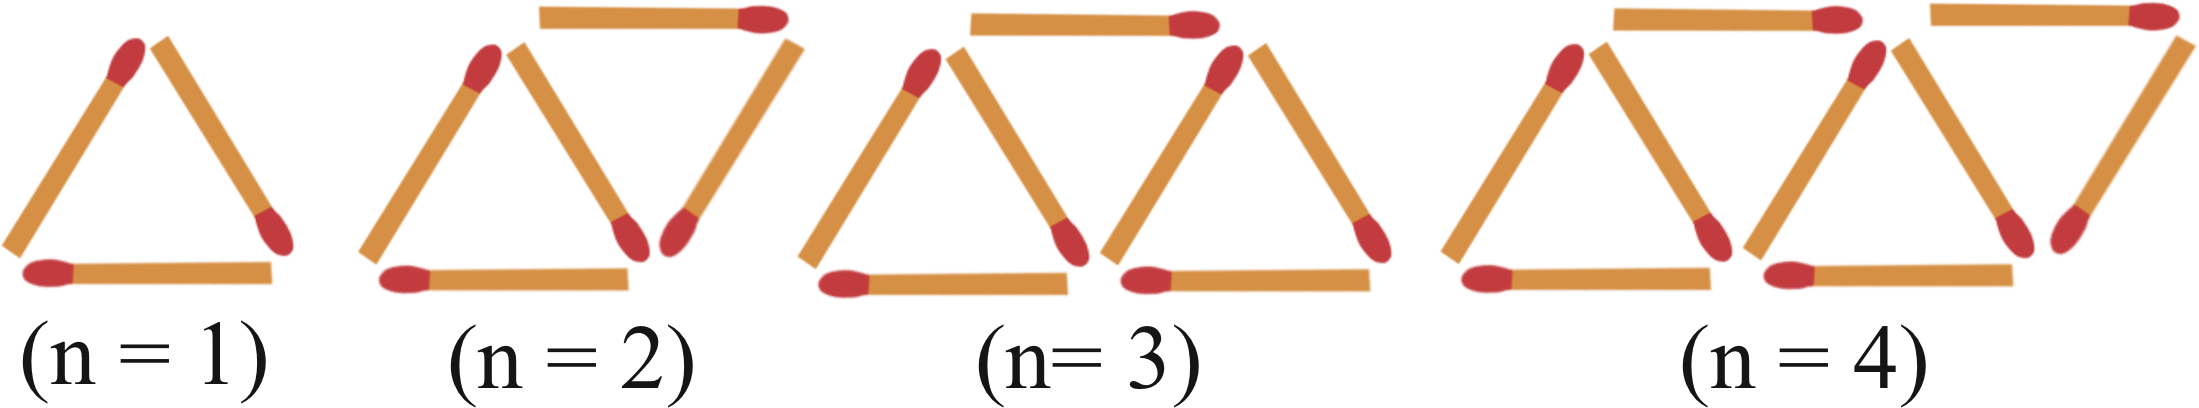
\includegraphics[width=\textwidth]{./ilustras-mat/Simulado_1-atividade_6.png}
\end{figure}

Seguindo o padrão da imagem, quantos palitos haverá na figura de $n = 8$?

\begin{multicols}{2}
\begin{escolha}

  \item 10

  \item 12

  \item 16

  \item 17

\end{escolha}
\end{multicols}

\num{7} Um objeto é lançado obliquamente. Sua trajetória é descrita pela
função $h(t) = - t^{2} + 5t$. Nessa função, $h(t)$ representa a altura, em
metros; \textit{t} representa o tempo em segundos. A quantos metros de altura
estará o objeto após 3 segundos do lançamento?

\begin{escolha}

  \item 1

  \item 2

  \item 4

  \item 6

\end{escolha}

\num{8} Rodrigo é prudente e sempre controla a velocidade do carro em suas
viagens. Recentemente ele fez o trajeto entre Porto Feliz e Cidade Alegre em 
2,5 horas, na  velocidade média de 80 km.

Se fizer a viagem de volta com velocidade média de 100 km/h, quanto tempo 
Rodrigo levará de Cidade Alegre a Porto Feliz?  

\begin{escolha}

  \item 1h30

  \item 2h 
  
  \item 2h40
  
  \item 3h

\end{escolha}

\num{9} Apesar dos corridas por aplicativos terem emplacado, há cidades que ainda
contam apenas com táxis convencionais. Em um dessas cidades, na corrida de 
táxi é cobrado um valor inicial fixo, chamado de bandeirada, mais a quantia
proporcional aos quilômetros percorridos. Se por uma corrida de 10 km são pagos
R\$ 34,50 e, por uma corrida de 4 km, R\$ 16,50, então o valor da bandeirada é

\begin{escolha}

  \item R\$ 7,50.

  \item R\$ 6,50.

  \item R\$ 5,50.

  \item R\$ 4,50.
\end{escolha}

\pagebreak
\num{10} A figura a seguir mostra uma circunferência, em que os arcos ADC e
AEB são congruentes e medem 150° cada um.

\begin{figure}[htpb!]
\centering
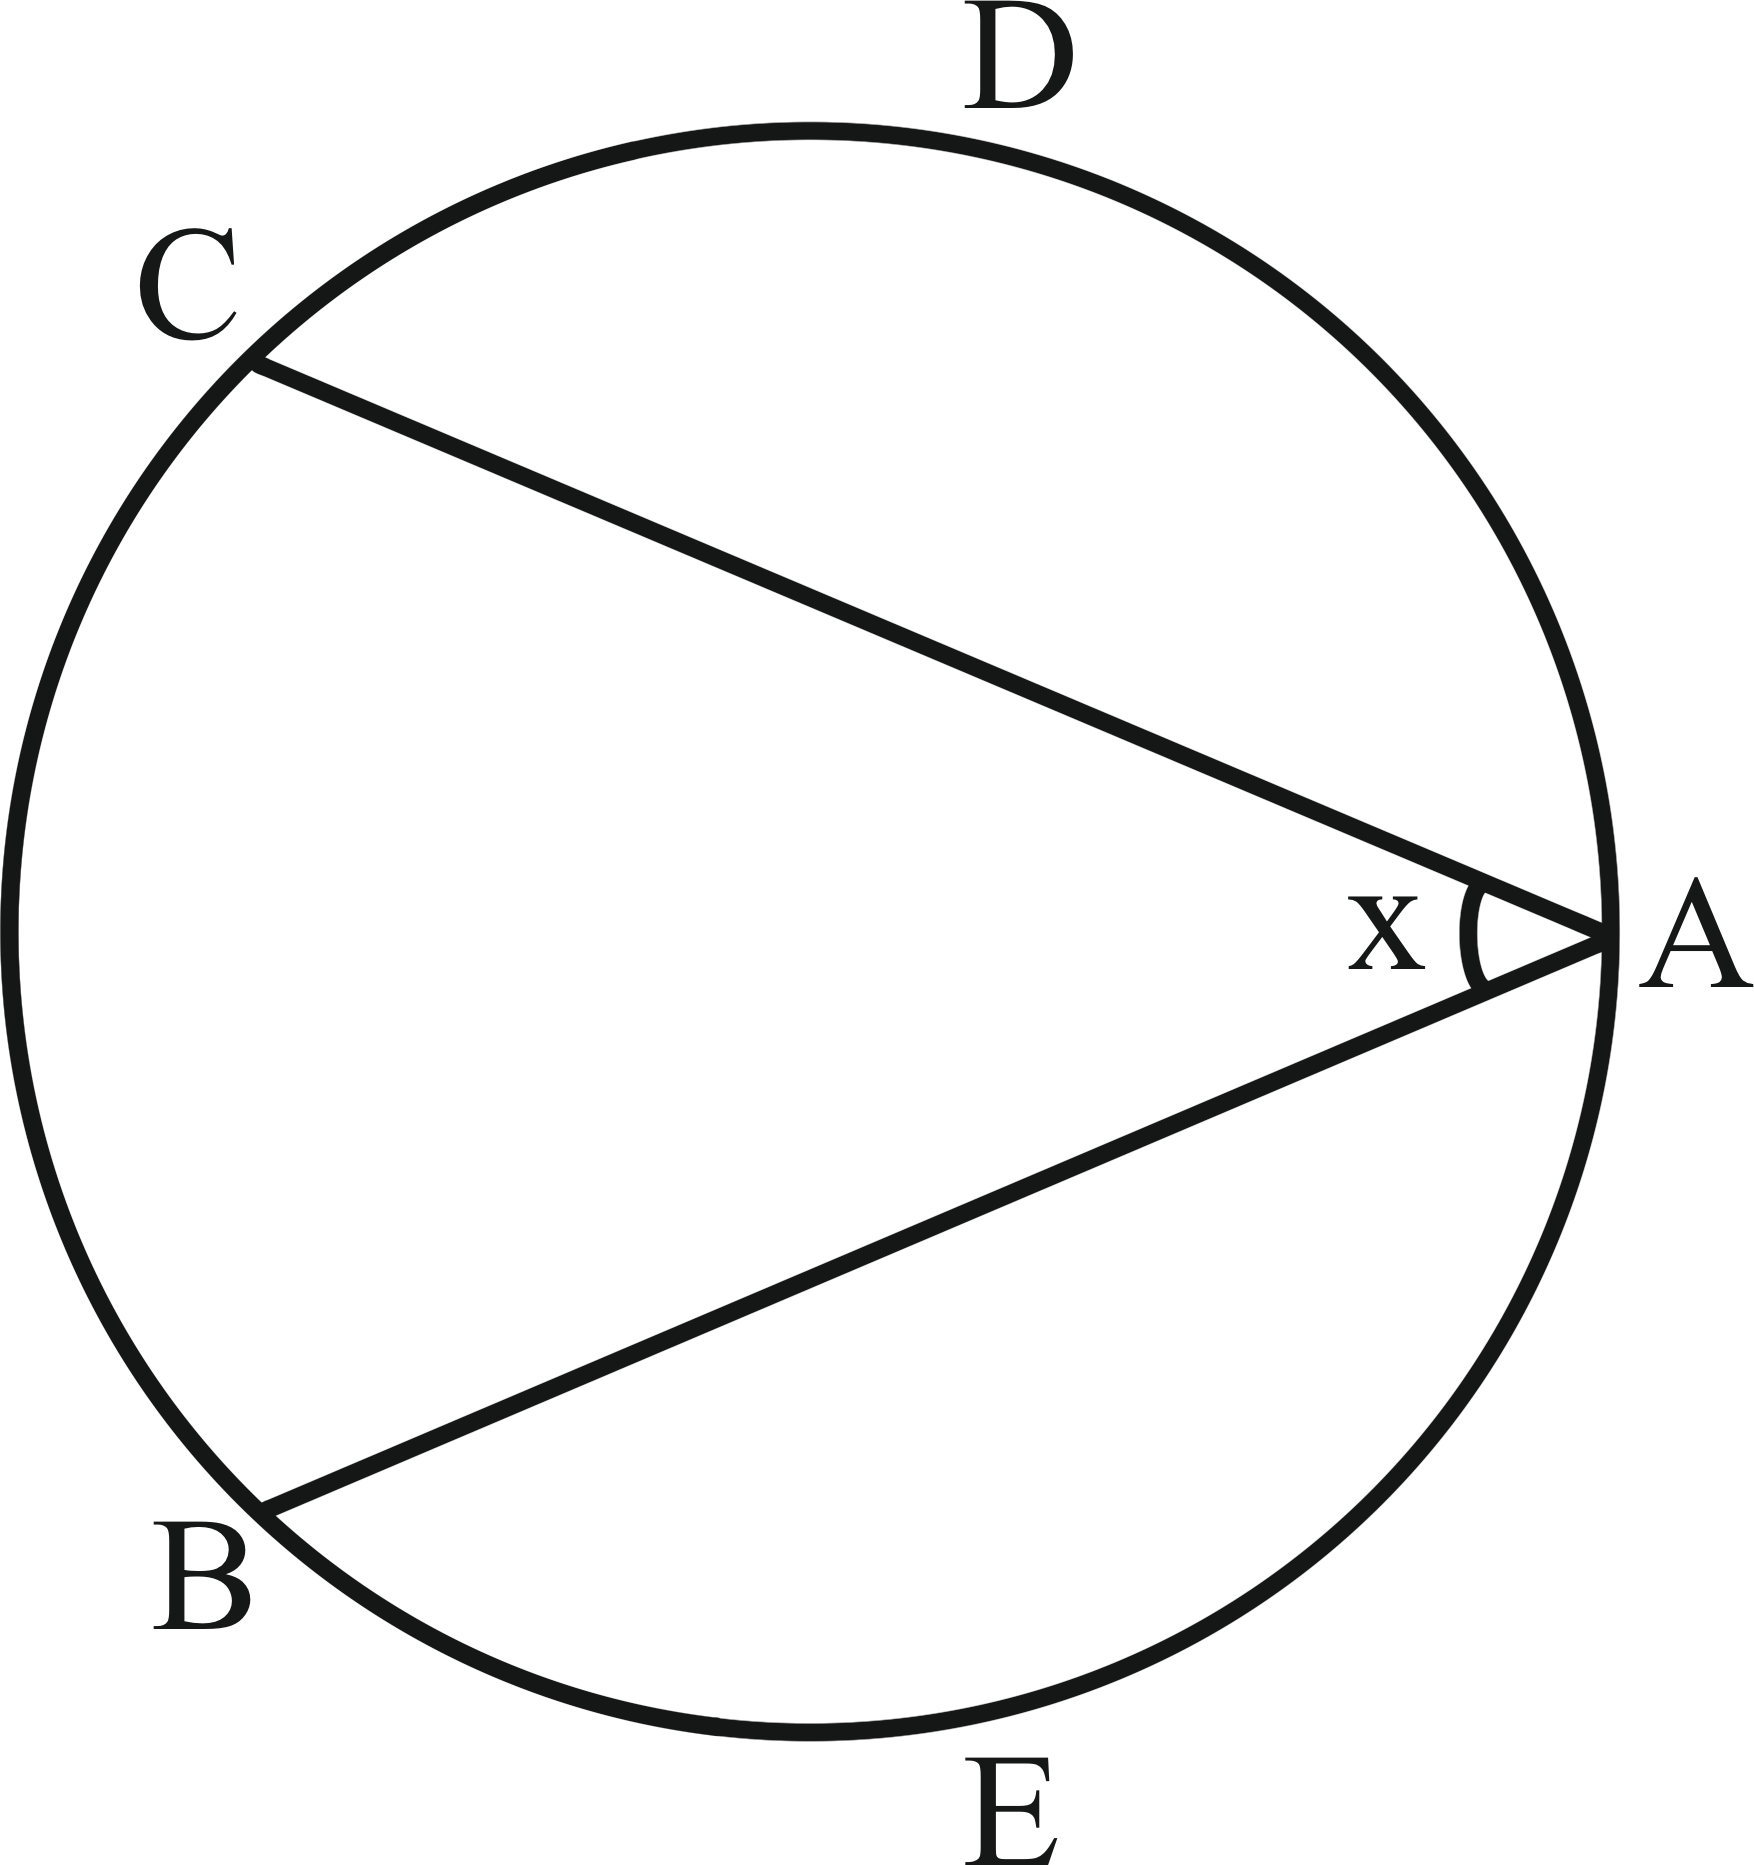
\includegraphics[width=.4\textwidth]{./ilustras-mat/Simulado_1-atividade_10.png}
\end{figure}

Qual o valor de x?

\begin{escolha}
  
  \item 10°

  \item 20°

  \item 30° 
  
  \item 40° 

\end{escolha}

\num{11} Na imagem a seguir, as retas \textbf{u}, \textbf{r} e \textbf{s} são paralelas
e cortadas por uma reta \textbf{t} transversal.

\begin{figure}[htpb!]
\centering
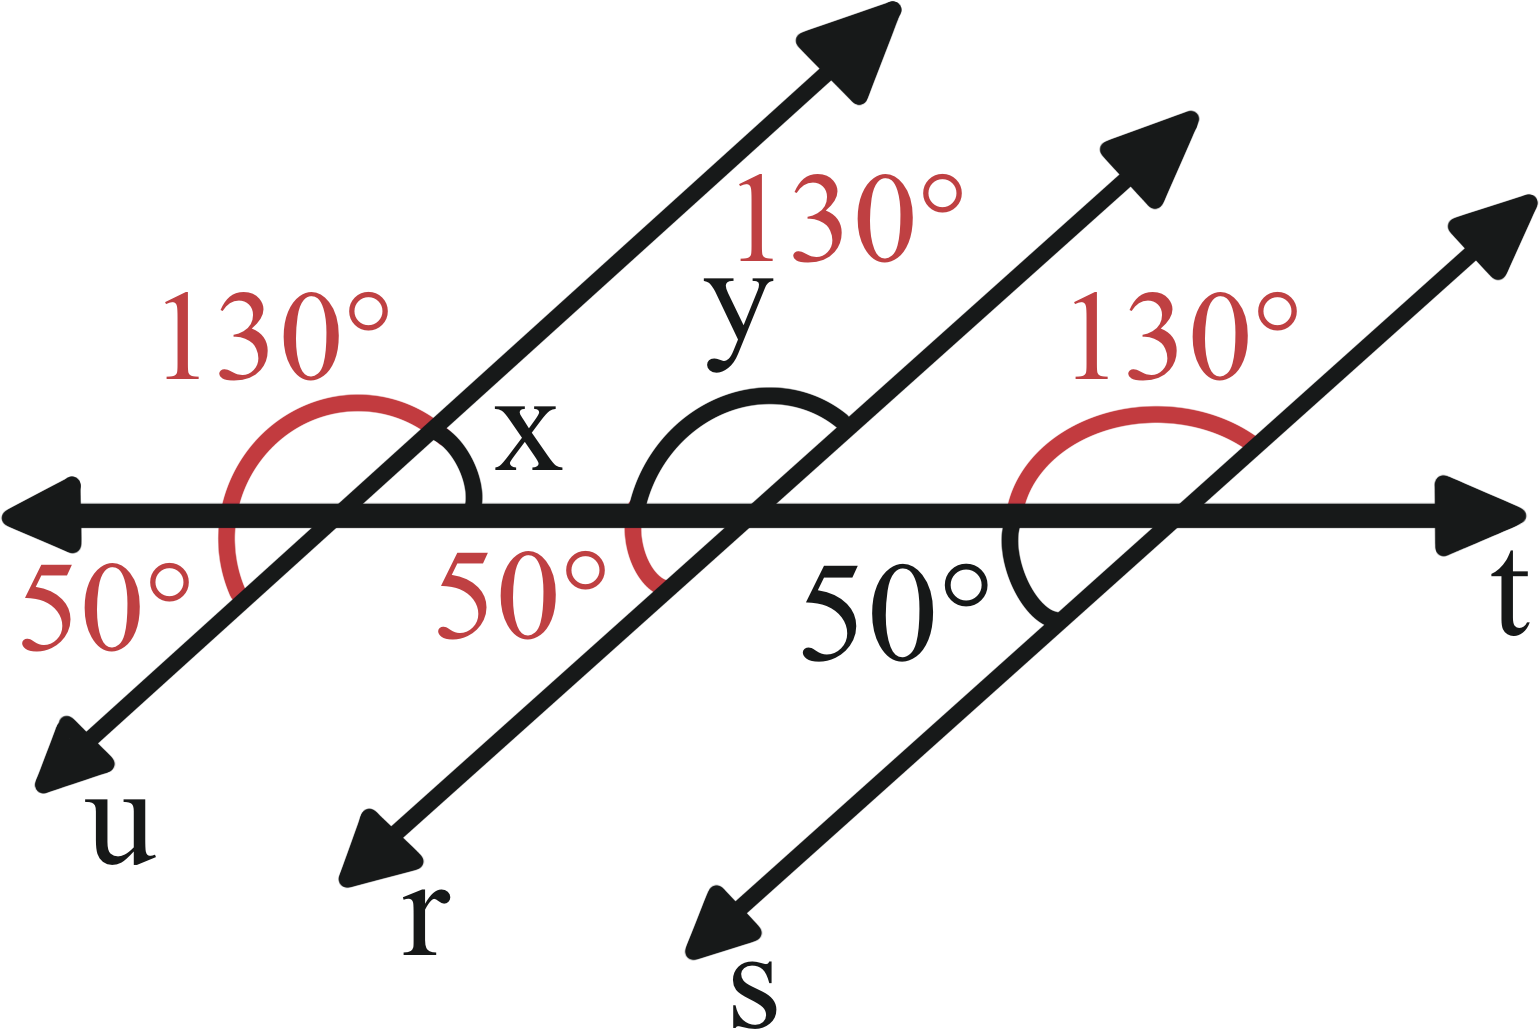
\includegraphics[width=.4\textwidth]{./ilustras-mat/Simulado_1-atividade_11_resposta.png}
\end{figure}

Qual o valor de x e y respectivamente?

\begin{escolha}

  \item 50° e 130°.

  \item 130° e 50°.

  \item 30° e 150°.

  \item 150° e 30°.

\end{escolha}

\num{12} O coordenador de uma escola de Ensino Médio fez uma pesquisa para
conhecer as carreiras que os alunos pretendem prestar no vestibular.

Após tabular os dados dos 170 estudantes entrevistados, chegou-se à
seguinte tabela:

\begin{longtable}[]{@{}lll@{}}
\toprule
Carreira & Masculino & Feminino\tabularnewline
\midrule
\endhead
Medicina & 17 & 20\tabularnewline
Direito & 8 & 16\tabularnewline
Administração & 12 & 22\tabularnewline
Fisioterapia & 8 & 16\tabularnewline
Outras & 25 & 26\tabularnewline
\bottomrule
\end{longtable}

Um desses estudantes é escolhido ao acaso. Ela é do sexo
feminino. A probabilidade de este estudante ter escolhido Administração
é de:

\begin{escolha}

  \item 7\%.

  \item 12,9\%.

  \item 16\%.

  \item 22\%.

\end{escolha}


\num{13} Em um concurso público, as notas finais dos candidatos foram
as seguintes:

\begin{longtable}[]{@{}ll@{}}
\toprule
Número de Candidatos & Nota Final\tabularnewline
\midrule
\endhead
7 & 6,0\tabularnewline
3 & 7,0\tabularnewline
4 & 9,0\tabularnewline
\bottomrule
\end{longtable}

Com base nessa tabela, a mediana das notas finais foi:

\begin{escolha}

  \item 6

  \item 6,5

  \item 7

  \item 9

\end{escolha}

\pagebreak
\num{14} Uma piscina retangular de 9,0 m x 12,0 m está cheia de água até 
a altura de 1,4 m. Um produto químico em pó deve ser misturado à água à razão
de um pacote para cada 3000 litros. O número de pacotes a serem comprados é:

\begin{escolha}

  \item 30

  \item 36

  \item 51

  \item 60

\end{escolha}

\num{15} Numa urna, foram colocados 10 cartões numerados de 1 a 10. Serão
sorteados, sem reposição, dois cartões. Qual a probabilidade
aproximada de os números presentes nos cartões sorteados serem pares?

\begin{escolha}

  \item 30\%

  \item 22\%

  \item 60\%

  \item 43\%

\end{escolha}

\num{16} Observe a imagem a seguir

\begin{figure}[htpb!]
\centering
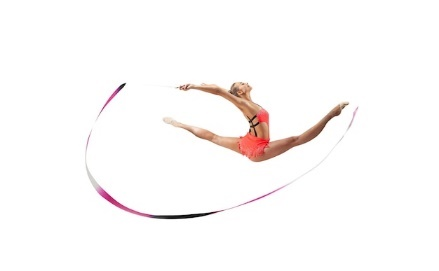
\includegraphics[width=.5\textwidth]{./imgs/img5.jpg}
%\caption{Disponível em: https://br.freepik.com/fotos-gratis/ginasta-ritmica-isolada-em-branco\_31843256.htm\#query=gin\%C3\%A1stica\%20art\%C3\%ADstica\&position=41\&from\_view=search\&track=ais.}
\end{figure}

A capacidade física utilizada no esporte apresentado é a

\begin{escolha}
\item força, pois a atleta está realizando um movimento com a sobrecarga da fita.

\item flexibilidade, pois a atleta está realizando uma abertura total das
pernas.

\item velocidade, pois a atleta deve movimentar rapidamente a fita.

\item resistência, pois a atleta está saltando tão alto quanto possível.
\end{escolha}

\pagebreak
\num{17} Leia o texto a seguir:

\begin{quote}
A tarde da última sexta foi um dia histórico para os skatistas
valadarenses, porque na ocasião a classe não só recebeu a notícia de
que a pista de skate da Feira da Paz será reformada como também pôde
falar sobre suas expectativas, discutir e sugerir propostas para o
projeto. {[}...{]}

O publicitário e skatista Diogo Lage foi à luta, procurou e indicou a
empresa especializada em pistas de skate para a Secretaria de Cultura, Esporte, Lazer e Turismo, levou o
arquiteto responsável pela elaboração dos projetos nas pistas e agora
está confiante. ``Com a reforma e revitalização do espaço, as famílias
poderão voltar a frequentar o local levando as crianças, e a comunidade
terá oportunidade de conhecer melhor o mais novo esporte olímpico. Com o
projeto concluído, os skatistas e o coletivo valadarense de skate farão a
Escolinha Social de Skate, que será uma oportunidade para tirar os
jovens do risco social da violência''.

\fonte{Prefeitura vai reformar a pista de skate. Prefeitura de Governador
Valadares. Disponível em:
https://www.valadares.mg.gov.br/detalhe-da-materia/info/prefeitura-vai-reformar-a-pista-de-skate/170101. com alterações.
Acesso em: 12 abr. 2023.}
\end{quote}

Com base no texto, os objetivos da reforma da pista de skate são

\begin{escolha}
\item lucrar com a prática de esportes urbanos e visibilizar a prática do skate.

\item formar atletas olímpicos no município e obter patrocínio privado para outros esportes.

\item atrair marcas que investem em skate e estimular a prática de esportes urbanos. 

\item atrair a comunidade para a prática do skate e usá-la como forma de prevenção à violência.
\end{escolha}

\num{18}  Leia a reportagem a seguir:

\begin{quote}
Respeito e disciplina são a base de tudo. As outras regras que você
precisa saber para acompanhar o judô estão aqui.

\textbf{Tatame}\\
As lutas acontecem em um tatame quadrado, com medidas que variam de 14 a
16 metros.

\textbf{Uniforme}\\
Os judocas devem usar um quimono. Um dos atletas recebe uma faixa
vermelha, além da própria faixa, e é chamado de \textit{aka} (vermelho). O outro
recebe uma faixa branca e é chamado de \textit{shiro} (branco).

\textbf{Duração} da luta\\
As lutas têm duração de 4 minutos para o feminino sênior e sub-21, e de
5 minutos para o masculino sênior.

\fonte{Infraero. Regras. Disponível em:
http://www.infraero.gov.br/judo/regras/. Acesso em: 22 fev. 2023.}
\end{quote}

\pagebreak
É possível afirmar que o judô passou pelo processo de esportivização,
porque, nessa arte marcial 

\begin{escolha}
\item não se distinguem categorias masculinas e femininas. 

\item o uso do quimono é condicionado à cor da faixa.

\item há padronização das regras e vestimentas.

\item valores éticos e morais são previstos no regulamento.
\end{escolha}

%Felipe: julgo que a versão original dessa questão era no mínimo discutível. A categorização do item a e a obrigatoriedade de uniforme do item b podem ser consideradas partes características do processo de esportivização, o que se confirma com o item c –– por isso mudei as alternativas.  


\num{19}
  \begin{quote}
  Os advogados de defesa de Willian da Silva Alves utilizaram leis da
  física para conseguir, na segunda-feira
  (23), a
  liberdade provisória do jovem, de 19 anos. Ele foi
  preso suspeito
  de assaltar um
  comércio em Cocal,
  267 km ao Norte
  de Teresina,
  após suposto reconhecimento da vítima. [...]
  Conforme a defesa de Willian,
  ele estava almoçando na casa da sogra, na Zona Rural de Cocal, no
  momento em que o roubo, no Centro do município, aconteceu. [...] Os
  advogados do jovem, Batista Filho Júnior e Bruno Portela, basearam a
  defesa no \textbf{princípio da impenetrabilidade da matéria}. [...]

\fonte{Ilanna Serena. G1 Notícias Piauí. Defesa usa fórmulas físicas para conseguir liberdade provisória de jovem no PI: ‘impossível estar em dois locais ao mesmo tempo’. Disponível em:
https://g1.globo.com/pi/piaui/noticia/2023/01/24/defesa-usa-formulas-fisicas-para-conseguir-liberdade-provisoria-de-jovem-no-pi-impossivel-estar-em-dois-locais-ao-mesmo-tempo.ghtml.
Acesso em: 24 fev. 2023.}
\end{quote}

Identifique, dentre as alternativas, aquela explica corretamente o conceito de impenetrabilidade.

\begin{escolha}
\item
  Qualquer matéria pode ser dividida em pedaços menores que os iniciais.
\item
  Um corpo tende a permanecer em seu estado natural até que outra força aja sobre ele.
\item
  Duas porções de matéria não podem ocupar o mesmo espaço ao mesmo tempo.
\item
  Toda matéria ocupa lugar no espaço.
\end{escolha}


\num{20}
\begin{quote}
Segundo dados do Instituto Nacional de Câncer (INCA), são esperados
60 mil novos casos de câncer de mama no Brasil em 2018; os números
crescem a cada ano e a neoplasia continua sendo a segunda maior causa
de morte entre as mulheres brasileiras. [...]
Fatores genéticos correspondem
à 12\% dos casos de câncer de mama e aumentam em 80\% as chances do
desenvolvimento deste tipo de câncer. [...]

\fonte{Hospital Oswaldo Cruz. Hereditariedade aumenta em 80\% as chances de se desenvolver câncer de mama. Disponível em:
https://www.hospitaloswaldocruz.org.br/imprensa/noticias/hereditariedade-aumenta-em-80-as-chances-de-se-desenvolver-cancer-de-mama/.
Acesso em: 24 fev. 2023.}
\end{quote}

\pagebreak
Uma doença hereditária é aquela que passa de pai pra filho no decorrer
das gerações. Identifique a alternativa que explica geneticamente como a
hereditariedade influencia no aparecimento do câncer.

\begin{escolha}
\item
  Os filhos herdam 100\% seu material genético dos genitores através das
  células germinativas, recebendo os genes com mutações cancerígenas.
\item
  Os filhos herdam 50\% do material genético dos genitores e os outros
  50\% são adquiridos no decorrer da vida, onde podem ocorrer mutações
  cancerígenas.
\item
  O câncer de mama está presente apenas no DNA de mulheres, sendo herdado
  100\% do DNA das mães.
\item
  Alterações genéticas cancerígenas como o câncer de mama são adquiridas
  na hora do parto, sendo herdadas exclusivamente dos pais.
\end{escolha}


\num{21}
\begin{quote}
  Com tamanho pouco superior ao da Lua, é o menor planeta do sistema solar, além de ser o mais próximo do Sol. Trata-se do menor
  dos planetas rochosos do sistema solar. Apresenta uma superfície repleta de crateras, assim como a Lua, o que se deve a uma
  finíssima atmosfera (exosfera) que o envolve. Com uma
  velocidade de mais de 170 km/h, trata-se também do
  planeta que viaja mais rapidamente pelo espaço (de onde vem seu nome)
  já que a velocidade de um planeta aumenta em função da sua proximidade
  da estrela que orbita.

\fonte{Fonte de pesquisa: National Geographic. Assim são os 8 planetas do sistema solar. Disponível
em: https://nationalgeographic.pt/ciencia/grandes-reportagens/3494-assim-sao-os-8-planetas-do-sistema-solar.
Acesso em: 22 fev. 2023.}
\end{quote}

A partir da leitura do texto e com base nos seus conhecimentos,
identifique o planeta ao qual o texto se refere.

\begin{escolha}
\item
  Mercúrio.
\item
  Vênus.
\item
  Plutão.
\item
  Saturno.
\end{escolha}
